\subsection{Systemmodell}
Vorwissen über das System findet im Systemmodell Anwendung. Mit der Überführungsfunktion $a$ wird der Folgezustand $\vec{x}_{t+1}$ aus dem aktuellem Zustand $\vec{x}_t$ abgeleitet. Der verwendete Zustandsraum $\mathbb{S} \times \IR^2$ beschreibt die position und Orientierung des Crawlers.


\begin{align*}
\vec{x}_{t+1} = a(\vec{x}_t) \oplus w_t
\end{align*}

Die Folge von Bewegungsbefehlen an den Crawler ist bekannt. Je nach Bewegungsbefehl ist die entsprechende Überführungsfunktion zu wählen:

\begin{equation}
    a(\vec{x}_t, command) = 
        \begin{cases}
            a_{fwd} \oplus w_{fwd},& \text{falls } command= fwd \\
            a_{left} \oplus w_{left},& \text{falls } command= left\\
            a_{right} \oplus w_{right},& \text{falls } comman= right
        \end{cases}
\end{equation}

Die tatsächliche ausgeführten Schritte variieren jedoch, auch für gleichbleibende Bewegungsrichtungen. Dies wir in Abbildung \ref{fig:moves} deutlich. Deswegen wird bei jedem Schritt zusätzlich ein Rauschterm $w_t$ addiert. Dies lässt sich in SE(2) durch die Multiplikation der dualen Quaternionen darstellen, was durch den $\oplus$-Operator ausgedrückt wird.
Die Schrittlängen und Drehungen wurden in einem Vorexperiment durch Tracking der LEDs mit der Deckenkamera aufgenommen. Es wurden drei SE(2)-Bingham-Verteilungen auf die gewonnen Daten angepasst, aus denen die jeweiligen $w_t$ zufällig gezogen werden.





\begin{figure}[ht]
	\centering
    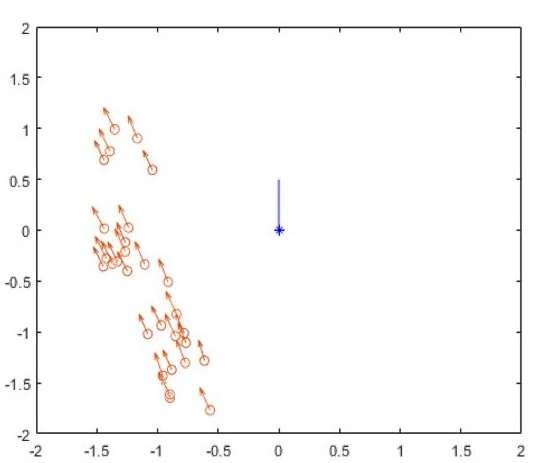
\includegraphics[width=.32\textwidth]{Images/links.jpg}
    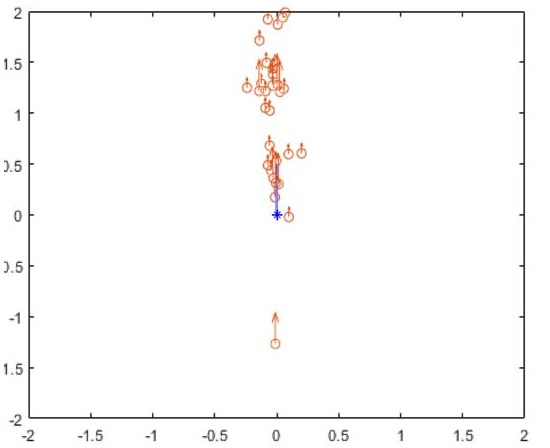
\includegraphics[width=.32\textwidth]{Images/vorne.jpg}
    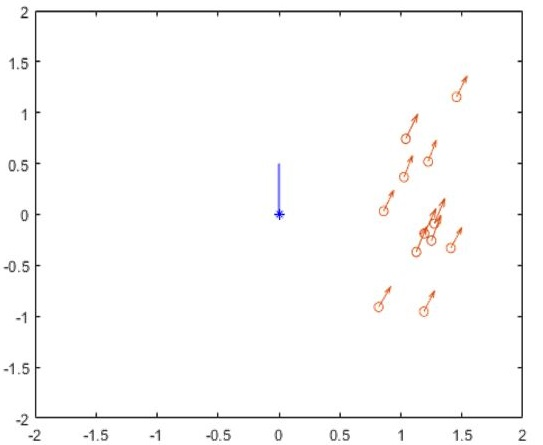
\includegraphics[width=.32\textwidth]{Images/rechts.jpg}
	\caption{Gemessene Verteilungen der Position und Rotation des Laufrobotters nach der Ausführung einer Bewegung. Blau ist der Ausgangszustand dargestellt. Die Zustände nach je einem Schritt in rot. Jede Verteilung wurde für einen der drei Bewegungsbefehle 'links', 'vorwärts' und 'rechts' mit einer Deckenkamera gemessen.}
	\label{fig:moves}
\end{figure}

Daraus werden die Erwartungswert und Varianz berechnet,und wir bezeichnen diese Datensätze als die echte Systemrauschen von Roboter.